\subsection{Media Agenda: differences between newspapers}

\par In this section we leave aside the Public Agenda and we study how the Media agenda varies when one consider the newspapers separately. 
In figure \ref{fig:news_agenda} we show the bump charts which belongs to each newspaper analogously to figure \ref{fig:all_agenda}.
The topics are the same introduced in the wordclouds of figure \ref{fig:topics_wordclouds}, but at computing the topics' weights the articles are separated by newspaper. 
We also show the radar plots showing the average distribution, as made in figure \ref{fig:topics_wordclouds}. 
\par In figure \ref{fig:news_agenda} we can see in a qualitative way the slightly differences between the newspapers' agendas.
For instance, we can see how \emph{Página 12} gave more importance to the topics \emph{Missing person} and \emph{Social leader}, while it did not pay too much attention to the \emph{Former Planning minister} as the others did.

% Jensen shannon distance of Dynamic way
\begin{figure}[h]
\centering
\includegraphics[width = \textwidth]{images/Fig5.pdf}
\caption{\textbf{Bump charts of newspapers' Agenda and radar plot of the average distributions.} The figure shows, in a qualitative way, the differences between the mentioned agendas, for instance, the greater interest of Página 12 (P12) in the \emph{Missing person}’s topic and its slightly lesser interest in the \emph{Former Planning minister} respect to the other newspapers.}
\label{fig:news_agenda}
\end{figure}

\subsubsection{Independent behavior}

\par In other to detect an independent behavior of a newspaper respect the others we again calculate the Jensen-Shannon distance between the newspapers agenda and the Media Agenda.
Note that this is the distance between the distributions of figure \ref{fig:news_agenda} and the top panel of figure \ref{fig:all_agenda}.
\par In figure \ref{fig:jensen_shannon_news} we show the Jensen-Shannon distance is a function of time.
We detect three points as outliers, although we discard the point \textbf{(b)} due to the low information of \emph{Infobae} in that period. 
The other two points belongs to a difference between \emph{Página 12} and the other newspapers. 
We interpret that the coverage of the topic \emph{Missing person} is the principal cause of the outliers.
\emph{Página 12} paid more attention to it than the Media Agenda at point \textbf{(a)} when the first notices of the Santiago Maldonado's disappearance before the primary elections, and in point \textbf{(c)} when a march two months after the disappearance took place, and had not the same coverage as the other march a month before (see section \ref{sec:Context}). Also, in point \textbf{(c)}, it can be seen a greater coverage of \emph{Página 12} in the topic \emph{Social leader} while the others seemed to be more interested in the topic \emph{Former Vice-President}.

% Jensen shannon distance of Dynamic way
\begin{figure}[h]
\centering
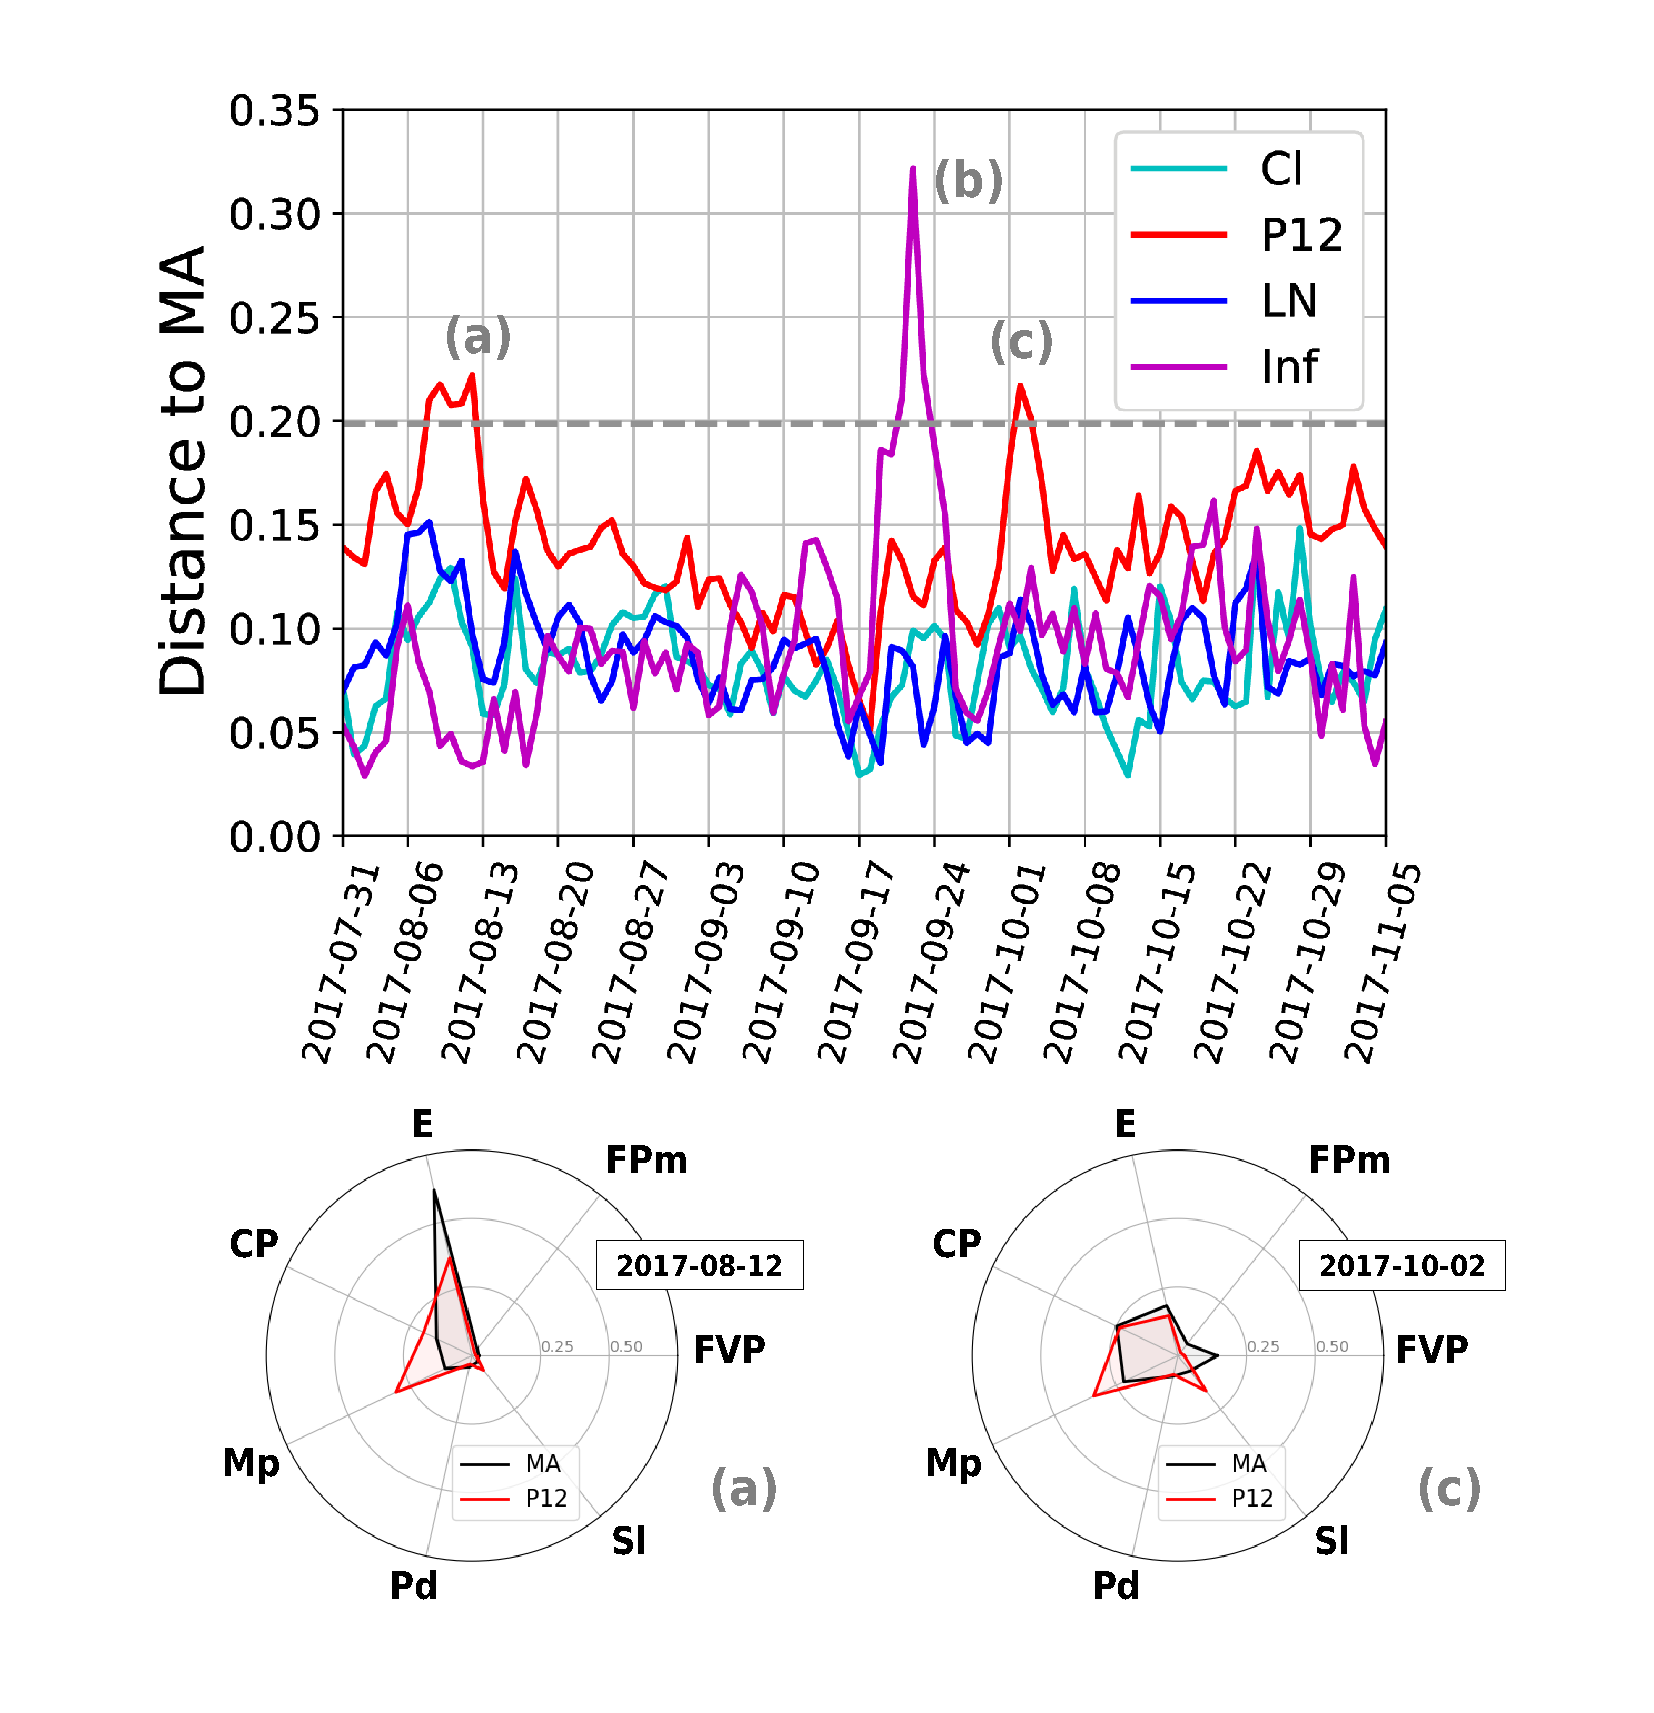
\includegraphics[width = \textwidth]{images/Fig6.pdf}
\caption{\textbf{Jensen Shannon distance between the newspapers’ agenda and the Media Agenda as a function of time.} \emph{Página 12} (P12) shows the more different behavior, motivated again by its interest in the \emph{Missing person} and \emph{Social leader} topics as can be seen in the radar plots which belongs to points (a) and (c). 
The anomalous behavior of \emph{Infobae} (Inf) at point (b) is due to few articles around that date in our database, therefore we ignore its radar plot.}
\label{fig:jensen_shannon_news}
\end{figure}

\subsubsection{Coverage bias}

\par The greater coverage in the topic \emph{Missing person} by \emph{Página 12} is even more clear if we inspect the temporal profile of the topic and compare the coverage given by each newspaper. A difference in the coverage is what it is called \emph{coverage bias}.
In figure \ref{fig:topics_temporal_profiles} we show the temporal profile of the topic \emph{Missing person} (panel (a)) and the topic \emph{Former Planning minister} in panel (b), as an example where the behavior is the opposite, as can be seen below.

\begin{figure}[h]
\centering
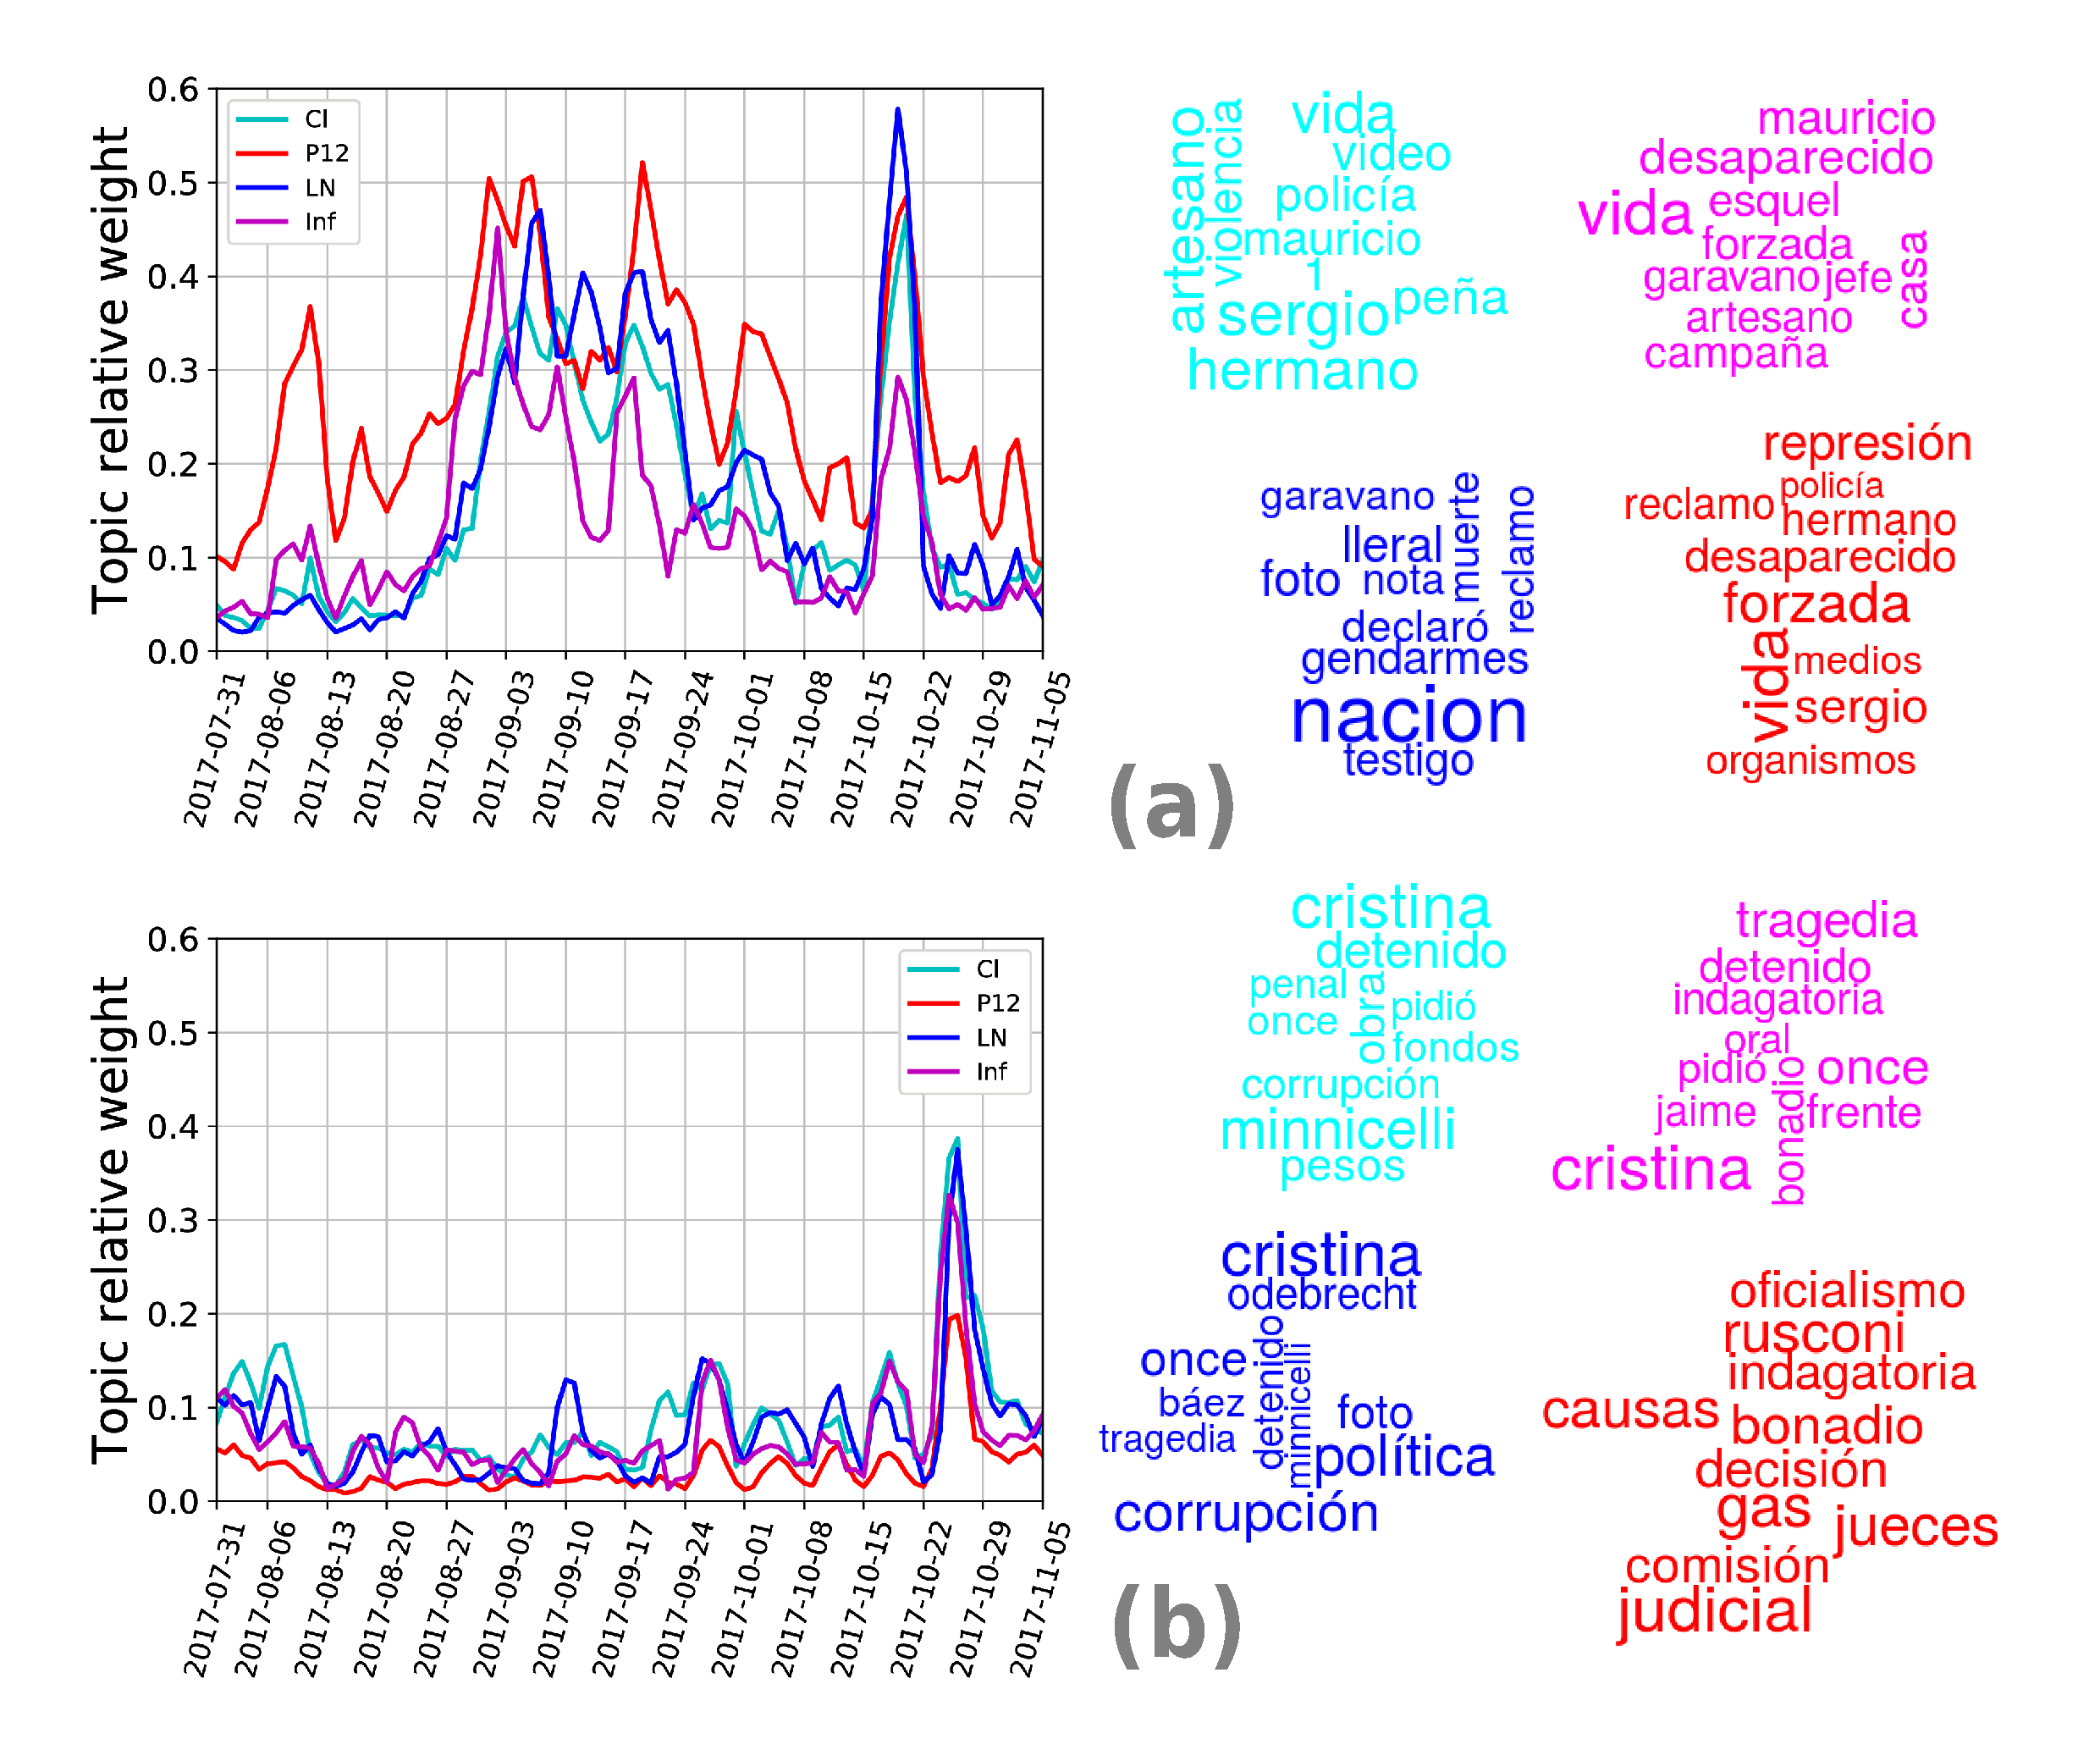
\includegraphics[width = \textwidth]{images/Fig7.pdf}
\caption{\textbf{Relative weight of the topics (a) \emph{Missing person}, and (b) \emph{Former Planning Minister}, and wordclouds of frequent newspapers' keywords}. We interpreted the differences shown in certain periods as an indicator of coverage bias. For instance, in figure (a) Página 12 pays a greater attention in the first days. In the wordclouds, we show which of the defining words are more frequently used by the corresponding newspaper. Most of them are less informative, but other seems to represent a first approximation in the study of framing.}
\label{fig:topics_temporal_profiles}
\end{figure}

\par From panel (a) of figure \ref{fig:topics_temporal_profiles}, we can see a more coverage of \emph{Página 12} respect the other newspapers at the first of the period. We can for instance quantify this difference by the median of the signals. If we focus in the period between July 31th and August 27th, the median of the topic relative weight for \emph{Página 12} is roughly 0.14 and this is statistically significant larger ($p < 10^{-7}$) than other medians, which are lower than 0.05.
Analyzing the same period, but in panel (b), we again can show that the median in \emph{Página 12}, which is roughly 0.01, is lower than the others, which oscillate around 0.05 ($p<10^{-3}$)
This quantification is proposed as method of studying coverage bias in the context of the methodology implemented in our work. 

\par Finally, in figure \ref{fig:topics_temporal_profiles} we also show wordclouds of topic's keywords but separate those that are most frequent mentioned by each newspaper, filtering the words that are common to all and basically define the factual details of the topic.
Although most words are less informative, some are interesting to inspect, for instance, the word \emph{represión} (repression) when \emph{Pagina 12} talks about the topic \emph{Missing Person} and the word \emph{Cristina} (Fernández de Kirchner) which is employed by all newspapers except \emph{Pagina 12} when talk about the topic \emph{Former Planning minister} (see section \ref{sec:Context}).
We don't go farther but we think that a more deeply study of topics' keywords is a first approximation in the study of framing, which will constitute the core of futures works.
